\section{Description}


We used various optics to build a Michelson Interferometer (a  complete list will be added at the end of this document.) We had to do several things during the process such as align the beam, mount some delicate optics, and test the end result. We mounted the He-Ne laser to the ULM-Tilt base and then placed it on one corner of the breadboard. We then had to assemble the silver mirrors onto their mounts. Using slips of paper to stabilize each mirror in its respective mount, we secured them in place. The mounts themselves were then attached to posts and placed in the following locations, shown in the diagram below.

\begin{figure}[!ht]
\centering
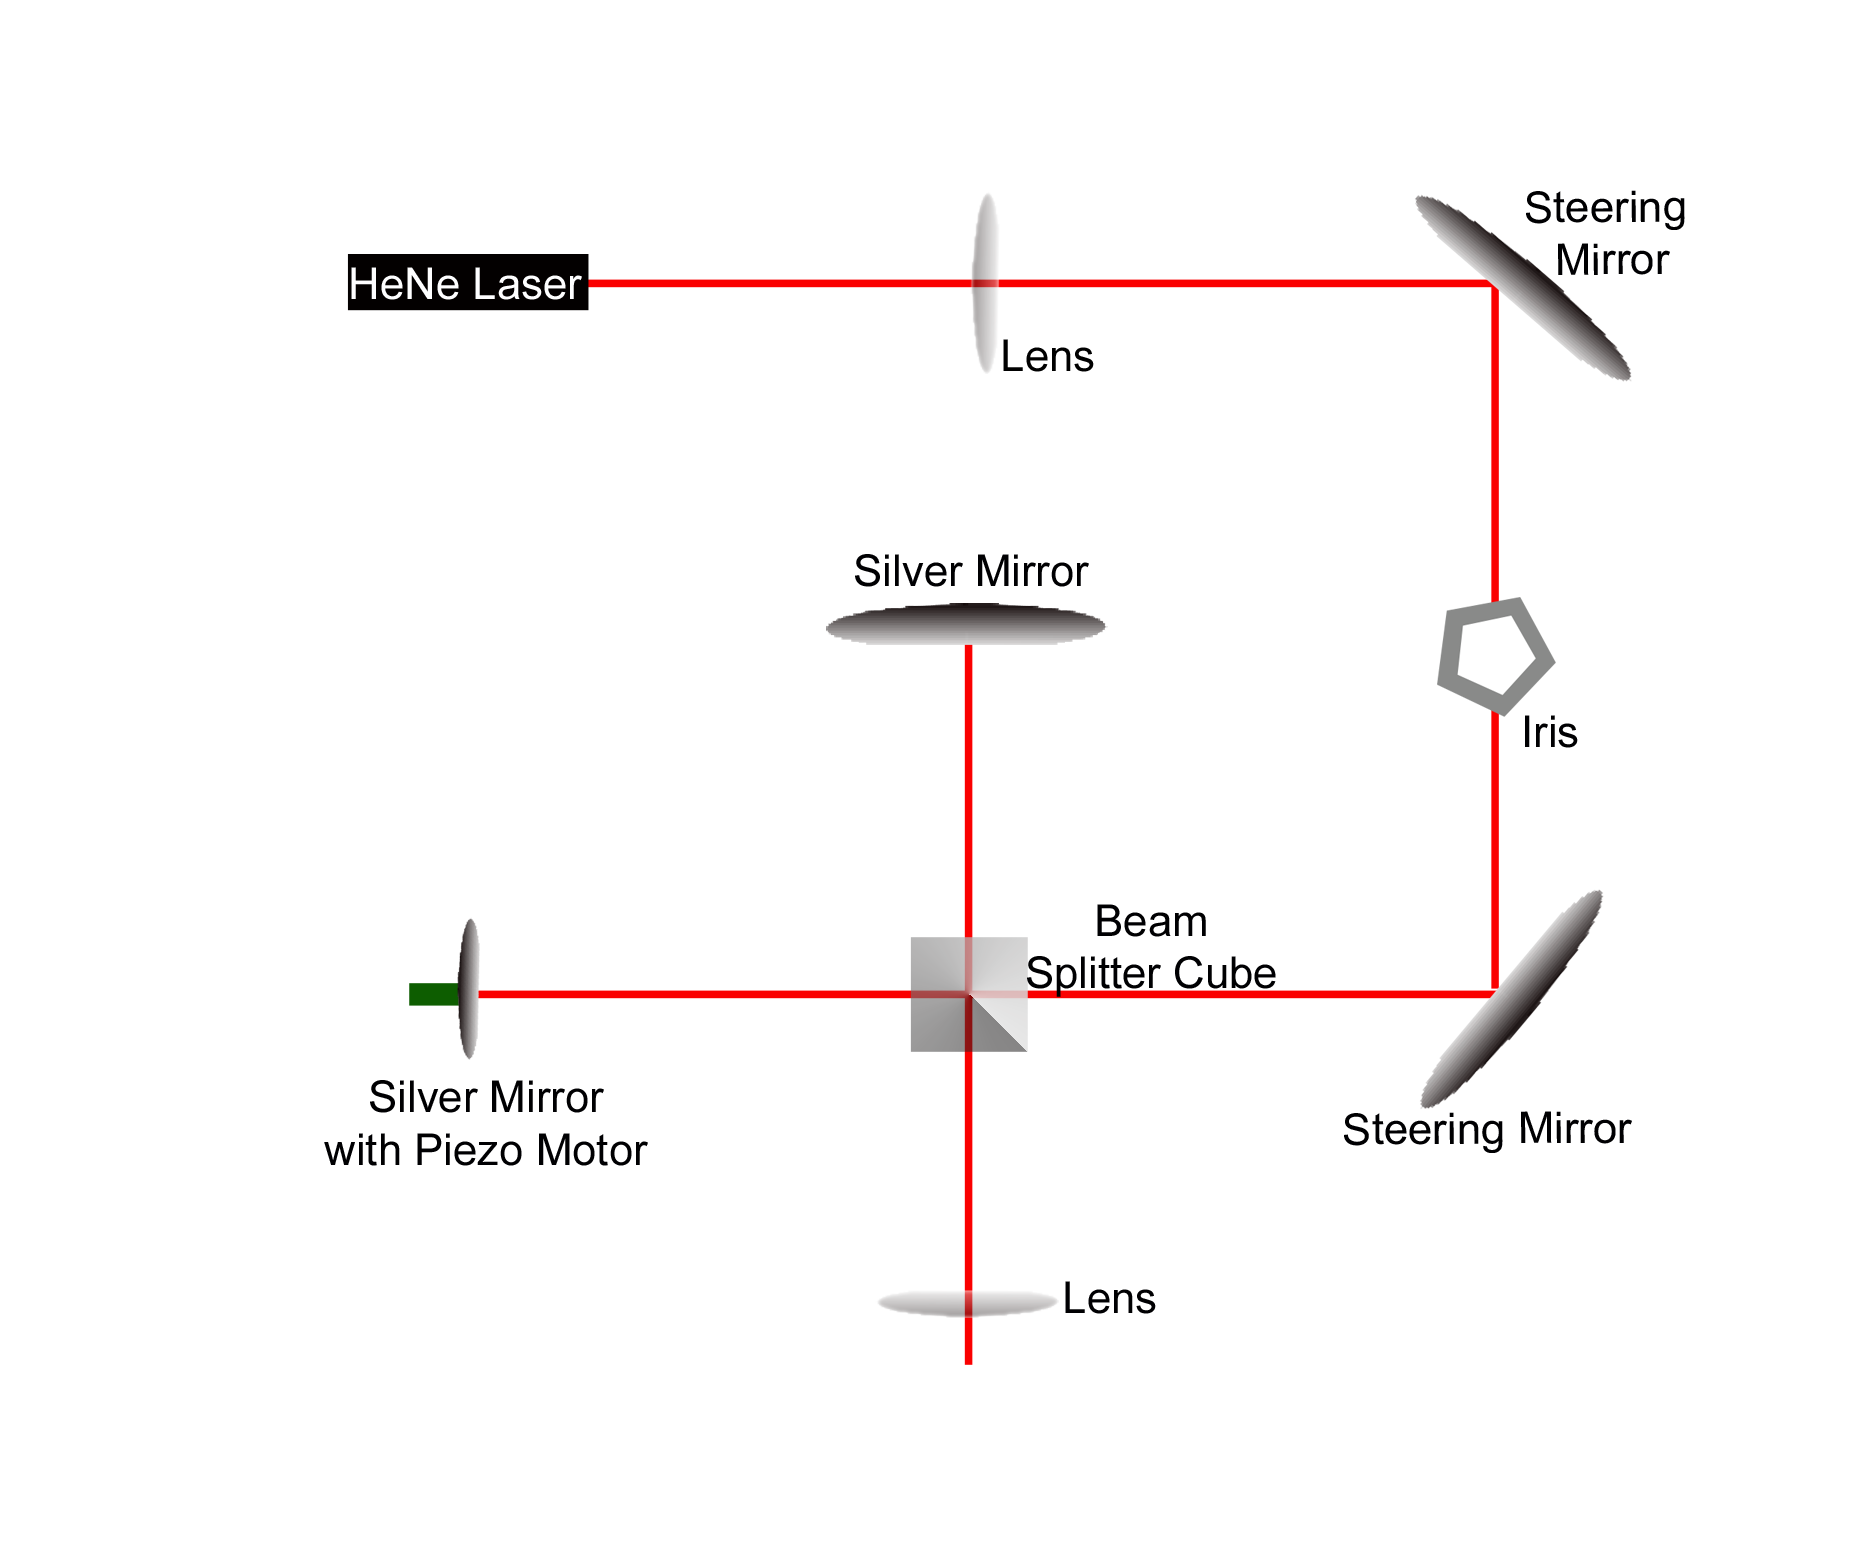
\includegraphics[width=5.5in]{interferometer}
\caption{Interferometer Diagram}
\label{fig:interferometer}
\end{figure}

The next major step we had to overcome was mounting the 0.5 in mirror on the piezo motor, but once in place we simply placed it on a post and set it aside.  Then we carefully mounted the beam splitter cube onto its mount with a small clamping arm. The mounted beam splitter was placed 4.5 inches away from Mirror 1 (the middle mirror in the diagram.) Using the same measurement we placed the Piezo Mirror to the left of the beam splitter.  After setting up this general layout, we turned on the laser to properly align it along the designated path.

%\subsection{Beam Alignment}
%
%
%  %    \item Laying out the Beam Path
%        \begin{enumerate}
%        \item Place Mirrors 1 and 2, and the Piezo Mirror as indicated by
%        Fig.~\ref{fig:interferometer}. These will form the primary beam path.
%        \item To ease alignment, attempt to direct the beam so that it lies over
%        the grid created by the breadboard holes.
%        \item Align the mirrors so that the beam strikes the center of each
%        mirror. Rough adjustments should be done by raising, lowering, or
%        rotating the post. Fine adjustments should be done using the adjustment
%        screw.
%        \end{enumerate}
%    \item Leveling the Beam
%    \label{step:leveling}
%        \begin{enumerate}
%        \item Place the iris halfway between the first two mirrors and shine the
%        beam through the iris. If the laser reflected off of the
%        second mirror does not retro-reflect through the iris onto the first mirror,
%        adjust the mirrors until it does.
%        \item Repeat this with the other mirrors until the entire beam path is
%        level.
%        \item When completed, the beam should travel from the He-Ne laser to the
%        Piezo mirror, then retro reflect back to the laser, aligned as close to
%        the aperture as possible.
%        \end{enumerate}
%    \item Introducing the Beam Splitter Cube
%        \begin{enumerate}
%		\item How to mount the Beam Splitter Cube.
%        \item Mount the Beam Splitter Cube on the breadboard between
%			  Mirror 2 and the Piezo Mirror. The Beam Splitter should split the laser beam perpendicular to the bean path.
%        \item Using the iris, verify that the beam is level between Mirror 2 and
%        the Piezo Mirror. If it is not, you may need to use the alignment screws
%        on the Kinematic Platform to level the Beam Splitter. You \emph{should
%        not} have to adjust the mirrors, as they were level previously.
%        \label{step:beamsplitter_level}
%        \end{enumerate}
%    \item Introducing Mirror 3 and Lens 2
%        \begin{enumerate}
%        \item Place Mirror 3 perpendicular to the beam path between Mirror 2 and
%        the Piezo Mirror, and an equal distance from the beam splitter as the
%        Piezo Mirror. Refer to Fig.~\ref{fig:interferometer} for clarification.
%        \item Verify that the center of Mirror 3 is the same height as that of
%        Mirrors 1 and 2, and all other optics.
%        \item Place Lens 2 perpendicular to the beam path between Mirror 2 and
%        the Piezo Mirror, opposite from Mirror 3. 
%        \item Verify that the center of Lens 2 is the same height as that of all
%        other optics.
%        \item Now using the iris, verify that the beam between Mirror 3 and Lens
%        3 is level. Again, if it is not level, use the alignment screws on the
%        Kinematic Platform for adjustment, as in
%        Step~\ref{step:beamsplitter_level}.  
%        \end{enumerate}
%    \end{enumerate}
%        
%\subsection{Further Beam Alignment}
%\label{sub:further}
%
%    \subsubsection{First Visualization}
%        \begin{enumerate}
%        \item Place a paper or screen vertically after Lens 2.
%        \item Depending on how well aligned your interferometer is, you should
%        see either two distinct beams, or a single beam with dark banding. If
%        you see two beams, use the alignment screws on Mirror 3 and the Piezo
%        Mirror to align these two beams on screen.
%
%            \emph{Alignment Tips}:
%            \begin{itemize}
%            \item If you see purely vertical banding, your misalignment lies
%            only in the horizontal direction.
%            \item Similarly, if you see purely horizontal banding, your
%            misalignment lies only in the vertical direction.
%            \item Diagonal banding is a combination of both vertical and
%            horizontal banding.
%            \item Curved banding is a good sign, as the misalignment is now
%            minimal.  You should seek the center of curvature of the bands.
%            \end{itemize}
%        \end{enumerate} 
%    \subsubsection{Test your interference}
%
%        The interferometer should be sensitive enough to pick up vibrations in
%        the table and breadboard generated by tapping. These would be seen as
%        dark bands moving on the screen.
%    \subsubsection{Achieving Optimum Focus}
%        \begin{enumerate}
%        \item Set the centerline height of Lens 1 to match all other
%        optics.
%        \item Place Lens 1 into the beam path between the He-Ne laser
%        and Mirror 1, and adjust their position to achieve the best focus
%        visible on the screen.
%        \item Mount the post holders to the board and verify that the beam path
%        is still level throughout the entire interferometer. (Refer to
%        Section~\ref{sub:preliminary} Step~\ref{step:leveling} if needed)
%        \end{enumerate}
%
%
%\subsection{Using the Photo Diode}
%\label{sec:photodiode}
%
%    \subsubsection{Introducing the Photo Diode}
%        \begin{enumerate}
%        \item Replace Lens 2 with the Photo Diode and center the beam on the
%        sensor.
%        \item Connect the Photo Diode to CH1 of the oscilloscope using a BNC
%        cable and the Variable Terminator set to the closest match possible to
%        your oscilloscope's impedance.
%        \item Turn on the voltage bias.
%        \item Now fringes can be seen as fluctuations in the signal.
%        \end{enumerate}